\chapter{Mathematical TRM Model and OGS Realization}
\label{chap:ogs-model}

\section{Purpose and Evidence Boundary}
\label{sec:purpose-evidence}

We use a two-layer description of the CD-A Niche 4 reference model.  The first
layer is the mathematical Thermo--Richards--Mechanics (TRM) model: domain, unknowns,
constitutive laws, boundary data, and initial state.  The second layer is the OGS
realization of that model through project-file blocks, XML parameters, mesh fields,
curves, time stepping, and VTU outputs.  This order is deliberate.  It fixes the
scientific model before we discuss how each field is passed into OGS or read from
OGS results.

The file-level evidence for the implementation is the transferred OGS project
\path{cd_a_open_niche_quad.prj}.  Its included process, process-variable,
parameter, media, time-loop, solver, and curve XML files are model inputs, not
literature sources; when a statement is model-specific, the relevant XML tag or
path is stated in the text or tables.  For the equations we use the OGS TRM
formulation without
vapor diffusion, the coupled THM notation of
\citet[Sec.~2.1--2.3, Eqs.~1, 7--9]{Wang2009THM}, and the OGS documentation
\citep[``Governing equations without vapor diffusion'']{OpenGeoSysTRMDocs}.
If the OGS project files contain an inactive parameter, commented block, or
implementation mismatch, we record it as a gate.  We do not promote such entries
into the active physics.

\section{Physical Setting and Modelled Phenomena}
\label{sec:physical-setting}

The CD-A experiment studies the coupled response of Opalinus Clay around twin niches
in the Mont Terri Rock Laboratory.  The relevant rock is a bedded claystone with
strong hydro-mechanical coupling, structural controls, and a near-niche excavation
damaged zone (EDZ).  The CD-A work focuses on humidity-driven water-content,
pressure, and deformation evolution in the formation
\citep[abstract]{Ziefle2021CDA}
\citep[abstract, Sec.~2, Table~1]{Ziefle2024Characterization}
\citep[abstract and Secs.~1--2]{WaterContentEDZ2024}.  Broader Mont Terri
studies show that Opalinus Clay stiffness, strength, pore-pressure response, and
damage-zone development depend on suction, bedding, in-situ stress, and fault or
fracture structure \citep[abstract, Secs.~2--3.3]{Amann2017Opalinus}.  EDZ
studies further show that hydraulic conductivity and fracture aperture can differ
by orders of magnitude from the intact claystone and can evolve through swelling,
closure, and self-sealing
\citep[abstract and Sec.~3.1.1]{Hale2021EDZ}
\citep[abstract, Secs.~2.1--2.5]{Marschall2017EDZ}.

The reference OGS model represents a controlled subset of this physics.  It includes
Richards pressure diffusion, capillary retention, relative permeability, porosity
storage, orthotropic linear elasticity, Biot/Bishop pore-stress coupling,
saturation-dependent swelling stress, and heat-balance terms.  It does not
explicitly represent vapor diffusion, discrete fracture flow, chemical alteration,
sealing/healing kinetics, staged excavation, or full three-dimensional fault
geometry.  These omissions matter near the niche and in the EDZ, but they remain
external gates or later scenario fields in this chapter.

\section{Mathematical Model}
\label{sec:mathematical-model}

\subsection{Domain, Unknowns, and State Fields}
\label{sec:domain-unknowns}

Let \(\Omega\subset\mathbb{R}^2\) be the current two-dimensional CD-A Niche 4 slice,
and let \(I=[0,t_{\mathrm{end}}]\) be the simulated time interval.  The primary
unknowns are displacement \(\uu:\Omega\times I\rightarrow\mathbb{R}^2\), liquid
pressure \(\pl:\Omega\times I\rightarrow\mathbb{R}\), and temperature
\(\TT:\Omega\times I\rightarrow\mathbb{R}\).  Liquid saturation, Darcy velocity,
stress, strain, swelling stress, and water-content proxies are state-dependent or
post-processed quantities.  Tables~\ref{tab:unknown-output-fields}--\ref{tab:intermediate-derived-fields}
separate the notation into unknown and output fields, material input fields, and
intermediate or derived quantities before they enter the equations.

\begingroup
\small
\setlength{\tabcolsep}{3pt}
\begin{longtable}{@{}L{0.20\textwidth} L{0.16\textwidth} L{0.16\textwidth} L{0.38\textwidth}@{}}
\caption{Unknowns and OGS output fields used in the reference model.}
\label{tab:unknown-output-fields}\\
\toprule
Field & Symbol & Unit & Mathematical meaning and OGS status\\
\midrule
\endfirsthead
\toprule
Field & Symbol & Unit & Mathematical meaning and OGS status\\
\midrule
\endhead
\bottomrule
\endlastfoot
Displacement &
\(\uu=(u_x,u_y)\) &
\(\mathrm{m}\) &
Primary mechanical unknown and run-local output field.  It describes deformation of
the continuum slice relative to the chosen numerical initial state.\\
Liquid pressure &
\(\pl\) &
\(\mathrm{Pa}\) &
Primary hydraulic unknown and run-local output field.  In the Richards convention
used here, negative liquid pressure means positive suction relative to the
gas/reference pressure.\\
Temperature &
\(\TT\) &
\(\mathrm{K}\) &
Primary thermal unknown in the full TRM process and run-local output field.  In the
active parametrization it is constrained to \(T_0=298.15\,\mathrm{K}\) throughout the
domain and time interval.\\
Liquid saturation &
\(\Sl\) &
-- &
Secondary OGS state/output field computed from pressure through the retention law.
It is the mobile OGS liquid occupancy of the pore volume, not total
hydrogen-bearing water in the clay.\\
\end{longtable}
\endgroup

\begingroup
\small
\setlength{\tabcolsep}{3pt}
\begin{longtable}{@{}L{0.20\textwidth} L{0.16\textwidth} L{0.16\textwidth} L{0.38\textwidth}@{}}
\caption{Material fields and constitutive inputs to the active model.}
\label{tab:material-input-fields}\\
\toprule
Input field or parameter & Symbol & Unit & Material meaning and OGS role\\
\midrule
\endfirsthead
\toprule
Input field or parameter & Symbol & Unit & Material meaning and OGS role\\
\midrule
\endhead
\bottomrule
\endlastfoot
Intrinsic permeability &
\(\KK(\xx)\) &
\(\mathrm{m^2}\) &
Material tensor controlling Darcy mobility before multiplication by relative
permeability and division by viscosity.  The current workflow supplies it through
the run-local mesh field \texttt{k\_i\_rd}.\\
Porosity &
\(\por(\xx)\) &
-- &
Continuum pore-volume fraction used in storage, thermal mixing, and the
model-side water-content proxy.  It is supplied through \texttt{n\_rd} and is fixed
at \(0.105\) in the current field package.\\
Elasticity tensor &
\(\CC\) &
\(\mathrm{Pa}\) &
Orthotropic linear-elastic stiffness used in the mechanical constitutive law.  It is
a fixed constitutive input, not a released field in the present workflow.\\
Biot coefficient and Bishop law &
\(\alpha_B\), \(b(\Sl)\) &
-- &
Fixed pore-pressure coupling inputs.  In the active XML, \(\alpha_B=1\) and
\(b(\Sl)=\Sl\).\\
Liquid properties &
\(\rho_l^0(\pl)\), \(\mu_l\) &
\(\mathrm{kg\,m^{-3}}\), \(\mathrm{Pa\,s}\) &
Liquid density and viscosity used in storage and Darcy mobility.  Under the active
isothermal constraint, density depends on pressure but not on temperature.\\
\end{longtable}
\endgroup

\begingroup
\small
\setlength{\tabcolsep}{3pt}
\begin{longtable}{@{}L{0.20\textwidth} L{0.16\textwidth} L{0.16\textwidth} L{0.38\textwidth}@{}}
\caption{Intermediate and derived quantities used by equations and observation operators.}
\label{tab:intermediate-derived-fields}\\
\toprule
Quantity & Symbol & Unit & Mathematical meaning\\
\midrule
\endfirsthead
\toprule
Quantity & Symbol & Unit & Mathematical meaning\\
\midrule
\endhead
\bottomrule
\endlastfoot
Capillary pressure &
\(\pc=-\pl\) &
\(\mathrm{Pa}\) &
Retention-curve argument under the active sign convention.\\
Relative permeability &
\(k_{\mathrm{rel}}(\Sl)\) &
-- &
Saturation-dependent mobility reduction in the liquid phase.  It is computed from
the fixed relative-permeability law, not fitted independently.\\
Darcy velocity and mass flux &
\(\vl\), \(\ql=\rho_l\vl\) &
\(\mathrm{m\,s^{-1}}\), \(\mathrm{kg\,m^{-2}\,s^{-1}}\) &
Derived hydraulic transport quantities.  They are not pore velocity unless divided
by an explicitly chosen pore-volume factor.\\
Strain and stress &
\(\eps(\uu)\), \(\sig\) &
--, \(\mathrm{Pa}\) &
Mechanical fields derived from displacement, orthotropic elasticity, swelling strain,
and Bishop/Biot pore-pressure coupling.\\
Swelling strain or stress contribution &
\(\eps^{\mathrm{sw}}\), \(p_{\mathrm{sw}}\) &
--, \(\mathrm{Pa}\) &
Saturation-dependent mechanical contribution used inside the active constitutive
law.\\
Volumetric water-content proxy &
\(\theta=\por\Sl\) &
-- &
Model-derived mobile-water proxy.  It needs an observation operator before it can be
compared with NMR, ERT, or Taupe/TDR.\\
\end{longtable}
\endgroup


We assume a single liquid phase in a porous solid, Richards-type capillary pressure
closure, no explicit gas-pressure unknown, and no active vapor diffusion.  The
reference body force is zero.  Temperature is retained in the full TRM statement
because it is an OGS primary variable and appears in density, heat storage, and
thermo-mechanical coupling
\citep[``Governing equations without vapor diffusion'' and ``Process variables'']{OpenGeoSysTRMDocs}.
Section~\ref{sec:isothermal-reduced-model} then records the reduced isothermal
model implied by the temperature initial and boundary entries in
\path{02_process_variables_TRM.xml} and \path{03_parameters_TRM.xml}.

\subsection{Liquid Flow, Retention, and Relative Permeability}
\label{sec:darcy-retention}

The liquid velocity is the Darcy velocity.  Here \(k_{\mathrm{rel}}\) is relative
permeability, \(\mu_l\) is liquid viscosity, \(\KK\) is intrinsic permeability,
\(\rho_l\) is liquid density, and \(\ql\) is liquid mass flux.  With the specific
body force disabled, the reference equation is
\begin{equation}
  \vl
  =
  -\frac{k_{\mathrm{rel}}(\Sl)}{\mu_l}\,\KK\,\grad \pl ,
  \qquad
  \ql=\rho_l\vl .
  \label{eq:darcy}
\end{equation}
The permeability tensor \(\KK\) is intrinsic permeability in \(\mathrm{m^2}\).  It
is not hydraulic conductivity.  Hydraulic conductivity is a derived quantity after
choosing liquid density, viscosity, relative permeability, and saturation state.  The
factor \(\por\Sl\) belongs to storage, thermal mixing, and the water-content proxy;
it is not part of the Darcy velocity in \eqref{eq:darcy}.

The active pressure convention is
\begin{equation}
  \pc := -\pl .
  \label{eq:capillary-pressure}
\end{equation}
Negative liquid pressure therefore means positive suction/capillary pressure
\revreplace{1}{under the gas/reference convention}{relative to the gas/reference pressure}{\annCommentOne}
used by the Richards formulation.  For \(\pc>0\), the
configured van Genuchten retention law is written with effective saturation \(S_e\).
The parameters \(S_{lr}\), \(S_{gr}\), \(m\), and \(p_b\) are the residual liquid
saturation, residual gas saturation, retention exponent, and pressure scale listed in
Table~\ref{tab:hydraulic-retention-parameters}:
\begin{equation}
  S_e(\pc)
  =
  \left[1+\left(\frac{\pc}{p_b}\right)^{1/(1-m)}\right]^{-m},
  \qquad
  \Sl
  =
  S_{lr} + (1-S_{lr}-S_{gr}) S_e ,
  \label{eq:vg-saturation}
\end{equation}
and the corresponding Mualem--van Genuchten relative-permeability law uses the lower
cutoff \(k_{\min}\):
\begin{equation}
  k_{\mathrm{rel}}(\Sl)
  =
  \max\!\left(
    k_{\min},
    S_e^{1/2}
    \left[1-\left(1-S_e^{1/m}\right)^m\right]^2
  \right).
  \label{eq:relative-permeability}
\end{equation}
\revadd{6}{Here \(S_e\) is the normalized retention variable, whereas \(\Sl\) is the
actual liquid saturation used by storage, water-content proxies, Bishop coupling,
and the relative-permeability evaluation.  \(S_{lr}\) shifts the lower liquid
saturation limit, and \(S_{gr}\) changes the conversion from \(S_e\) to \(\Sl\);
with the current \(S_{gr}=0\), it is still part of the formula but does not add a
separate gas-residual correction.}{\annCommentSix}
This closure follows the standard van Genuchten and Mualem forms
\citep[p.~892, Eqs.~2--3 and p.~893, Eq.~8]{VanGenuchten1980}
\citep[pp.~513--515, Eqs.~1--2, 14, and 21]{Mualem1976}.  In the present workflow
these retention and relative-permeability parameters are fixed model structure, not
varied calibration fields; their values are declared in
\path{04_2_media_twophase.xml}.

\begingroup
\small
\setlength{\tabcolsep}{3pt}
\begin{longtable}{@{}L{0.20\textwidth} L{0.16\textwidth} L{0.23\textwidth} L{0.31\textwidth}@{}}
\caption{Parameters introduced by the Darcy, retention, and relative-permeability equations.}
\label{tab:hydraulic-retention-parameters}\\
\toprule
XML name or law & Symbol & Active value & Role in Equations~\eqref{eq:darcy}--\eqref{eq:relative-permeability}\\
\midrule
\endfirsthead
\toprule
XML name or law & Symbol & Active value & Role\\
\midrule
\endhead
\bottomrule
\endlastfoot
\texttt{k\_i}/\texttt{k\_i\_rd} & \(\KK\) &
Baseline tensor \(\begin{bmatrix}1.0&0\\0&0.4\end{bmatrix}10^{-19}\,\mathrm{m^2}\);
current OGS mesh field varies magnitude &
Intrinsic permeability tensor in Darcy velocity.\\
\texttt{eta} & \(\mu_l\) &
\(1.0\times10^{-3}\,\mathrm{Pa\,s}\) &
Liquid viscosity in Darcy mobility.\\
VG saturation law & \(S_{lr},S_{gr},m,p_b\) &
\(0.1,0,0.45,10\,\mathrm{MPa}\) &
Retention curve \(S_l(p_c)\) with \(p_c=-p_l\).\\
VG relative permeability & \(k_{\mathrm{rel}}\), \(k_{\min}\) &
same residual saturations and \(m=0.45\), with \(k_{\min}=10^{-25}\) &
Unsaturated mobility reduction multiplying \(\KK/\mu_l\).\\
\end{longtable}
\endgroup


\subsection{Liquid Mass Balance}
\label{sec:mass-balance}

The no-vapor liquid mass equation can be written as follows.  Overdots denote time
derivatives.  The coefficient \(\beta_l\) is the pressure-derivative slot associated
with the liquid-density law, \(\alpha_B\) is the Biot coefficient, \(\alpha_T^s\) is
the solid thermal-expansivity parameter, and \(Q_H\) is the hydraulic source slot:
\begin{equation}
\left(
  \Sl\beta_l
  - \por\frac{\partial \Sl}{\partial \pc}
\right)\rho_l\,\dot{\pl}
-
\Sl
\left(
  \frac{\partial \rho_l}{\partial \TT}
  + \rho_l(\alpha_B-\Sl)\alpha_T^s
\right)\dot{\TT}
+
\divv(\rho_l\vl)
+
\Sl\alpha_B\rho_l\,\divv\dot{\uu}
= Q_H .
\label{eq:mass-balance}
\end{equation}
The equation shows why permeability, retention, porosity, density, temperature, and
mechanical volumetric strain cannot be interpreted independently.  In particular,
changing the boundary pressure curve or the retention law can mimic a change in
permeability through the desaturation timing.  The active XML does not add a
separate hydraulic source term, so \(Q_H=0\) in the checked baseline and is retained
only as the standard equation slot.  Vapor transport is also absent from this
no-vapor mass balance \citep[``Governing equations without vapor diffusion'']{OpenGeoSysTRMDocs}.

The liquid-density law is kept in its full TRM XML form,
\revreplace{10}{pressure- and temperature-dependent}{but the active run later
reduces it to the constant-temperature pressure law}{\annCommentTen}:
\begin{equation}
  \rho_l(\TT,\pl)
  =
  1095
  \left[
    1
    -5\times 10^{-4}(\TT-298.15)
    +3.2\times10^{-10}(\pl-7.5\times10^6)
  \right].
  \label{eq:liquid-density}
\end{equation}
Thus pressure storage, saturation storage, thermal density coupling, and mechanical
volumetric coupling belong to the full TRM statement.  \revadd{4}{The paper keeps
this equation because it is the checked OGS source form; no thermal calibration or
temperature-driven evolution is active in the current comparison.}{\annCommentFour} Under the current active
temperature constraints, the temperature terms reduce as stated in
Section~\ref{sec:isothermal-reduced-model}.

\begingroup
\small
\setlength{\tabcolsep}{3pt}
\begin{longtable}{@{}L{0.20\textwidth} L{0.16\textwidth} L{0.25\textwidth} L{0.29\textwidth}@{}}
\caption{Parameters introduced by the liquid mass balance and density law.}
\label{tab:liquid-mass-parameters}\\
\toprule
XML name or law & Symbol & Active value & Role in Equations~\eqref{eq:mass-balance}--\eqref{eq:liquid-density}\\
\midrule
\endfirsthead
\toprule
XML name or law & Symbol & Active value & Role\\
\midrule
\endhead
\bottomrule
\endlastfoot
\texttt{phi}/\texttt{n\_rd} & \(\por\) &
\(0.105\) in the current field package &
Porosity in liquid storage, retention derivative, thermal mixing, and
\(\theta=\por S_l\).\\
liquid density law & \(\rho_l(T,p_l)\) &
\(1095[1-5\times10^{-4}(T-298.15)+3.2\times10^{-10}(p_l-7.5\times10^6)]\) &
Full TRM density law.  Under the active isothermal constraint it reduces to
\(\rho_l^0(p_l)\) in Equation~\eqref{eq:isothermal-density}.\\
pressure slope in liquid density law & \(\beta_l\) &
\(3.2\times10^{-10}\,\mathrm{Pa}^{-1}\) relative pressure slope in the linear density law &
Used in the pressure-storage slot of Equation~\eqref{eq:mass-balance}; not a
separately released calibration parameter.\\
\texttt{biot} & \(\alpha_B\) &
\(1\) &
Couples volumetric strain and pore pressure to hydraulic storage and mechanics.\\
solid thermal expansivity & \(\alpha_T^s\) &
\texttt{CTE}=1254.74 in XML &
Appears in the thermal-coupling term of Equation~\eqref{eq:mass-balance}; value and
unit remain the CTE provenance caveat recorded in Table~\ref{tab:thermal-parameters}.\\
hydraulic source & \(Q_H\) &
No separate active source in the process file &
Retained as the standard equation slot, but not used as an additional forcing term.\\
\end{longtable}
\endgroup


\subsection{Quasi-static Mechanics}
\label{sec:mechanics-equation}

The mechanical balance is quasi-static.  The vector \(\bm{f}\) is the body-force
term, \(b(\Sl)\) is the Bishop saturation factor, and \(\alpha_B\) is the Biot
coefficient:
\begin{equation}
  \divv\!\left(\sig - b(\Sl)\alpha_B\pl\II\right) + \bm{f} = \bm{0}.
  \label{eq:momentum}
\end{equation}
The Bishop stress factor \(b(\Sl)\) represents the saturation-dependent weighting of
the pore-pressure term in unsaturated effective stress
\citep[bibliographic record, no DOI found]{Bishop1959EffectiveStress}.  For the
reference setup, the OGS Bishop law has exponent one and the Biot coefficient is
one, so \(b(\Sl)=\Sl\) and \(\alpha_B=1\) after substitution
\citep[TRM momentum equation and media-property table]{OpenGeoSysTRMDocs}; the
same values are declared by \texttt{BishopsPowerLaw} and \texttt{biot} entries in
\path{04_2_media_twophase.xml} and \path{03_parameters_TRM.xml}.  We keep the
symbolic form in \eqref{eq:momentum} because it makes the coupling assumptions
explicit.

The effective stress follows orthotropic linear elasticity with the thermal strain
term and the active OGS swelling-stress contribution:
\begin{equation}
  \sig
  =
  \CC:
  \left(
    \eps(\uu)
    -\eps^{\mathrm{th}}(\TT)
  \right)
  + \sig^{\mathrm{sw}}(\Sl),
  \qquad
  \eps(\uu)=\frac{1}{2}\left(\grad\uu+\grad\uu^\top\right).
  \label{eq:constitutive-mechanics}
\end{equation}
\revadd{8}{We therefore treat \(\sig^{\mathrm{sw}}\), not an independently
specified \(\eps^{\mathrm{sw}}\), as the active OGS object.}{\annCommentEight}
\revnote{18}{\pdfAnnComment{1}{markup on the swelling term}{The markup is addressed
by the same mechanics edit: the paper no longer treats swelling as an independent
strain law, but as the active OGS swelling-stress contribution in
\eqref{eq:constitutive-mechanics} and \eqref{eq:swelling-stress-rate}.}}
\revnote{19}{\pdfAnnComment{2}{z OGS kodu to vypada, ze se prispevek swellingu
pocita rovnou do stressu a ne do deformaci, jistota to neni}{Accepted.  The
reviewed equation states \(\sig^{\mathrm{sw}}(\Sl)\) as a stress contribution and
records the evidence boundary as the checked OGS implementation.}}
In each material direction, the configured saturation-dependent swelling-stress-rate
law is represented schematically by
\begin{equation}
  \dot{\sigma}^{\mathrm{sw}}_i
  =
  -\lambda_i p_i S_e^{\lambda_i-1}\dot S_e,
  \qquad
  \frac{\Delta\sigma^{\mathrm{sw}}_i}{\Delta t}
  =
  -\lambda_i p_i S_e^{\lambda_i-1}\frac{\Delta S_e}{\Delta t}.
  \label{eq:swelling-stress-rate}
\end{equation}
The checked XML gives \(p_i=1.0\,\mathrm{MPa}\) in all directions and exponent
\(\lambda_i=1\), with the saturation limits recorded in
Table~\ref{tab:mechanical-parameters}.
\revnote{39}{\pdfAnnComment{22}{highlight on the fixed \(1\,\mathrm{MPa}\)
swelling-pressure statement}{The highlighted value is treated as a checked XML
material input, not as a calibrated or published swelling-pressure claim.}}
\revadd{40}{The \(1.0\,\mathrm{MPa}\) value is therefore a checked OGS/XML material
input, not a literature-calibrated swelling pressure; changing it would be a
separate mechanics model-change decision.}{\pdfAnnComment{23}{odkud se vzal 1Mpa?}{The
paper now states the provenance boundary directly: the number comes from the active
XML input and remains a model-change decision if collaborators want a calibrated swelling
law.}}
\revadd{3}{This is a two-dimensional slice model.  The orthotropic stiffness values
come from the source OGS setup and are used as fixed in-plane constitutive data
for the current slice; out-of-plane stress assumptions, true 3D transfer of
elastic parameters, and excavation unloading are separate mechanics gates rather
than active calibration variables.}{\annCommentThree}
\revnote{37}{\pdfAnnComment{20}{ve skutecnosti jeste parametry pro swelling}{The
mechanics text and material tables now include the swelling pressure, exponent, and
saturation limits as fixed mechanical inputs alongside elasticity.}}
\revnote{38}{\pdfAnnComment{21}{potrebujeme vedet, plus prestress}{The bedding-angle
question remains separated from prestress.  Tensor orientation is a structural
gate, while prestress requires its own magnitude, angle or principal directions,
sign convention, and excavation-reference state.}}
The checked OGS input sets the specific body force to zero, so \(\bm{f}=\bm{0}\) in
the active baseline.  This is not a staged excavation model.  The current mechanics
model starts from the
already open two-dimensional geometry and has no active initial stress tensor or
active top load.  Any future mechanical residual therefore requires a separate
decision about prestress, excavation unloading, and the reference displacement
state.  This follows directly from \path{01_processes_TRM.xml}, where
\texttt{initial\_stress} is commented out, and from
\path{02_process_variables_TRM.xml}, where the top-load Neumann block is commented
out.

\begingroup
\small
\setlength{\tabcolsep}{3pt}
\begin{longtable}{@{}L{0.20\textwidth} L{0.16\textwidth} L{0.25\textwidth} L{0.29\textwidth}@{}}
\caption{Parameters introduced by the quasi-static mechanics equations.}
\label{tab:mechanical-parameters}\\
\toprule
XML name or law & Symbol & Active value & Role in Equations~\eqref{eq:momentum}--\eqref{eq:constitutive-mechanics}\\
\midrule
\endfirsthead
\toprule
XML name or law & Symbol & Active value & Role\\
\midrule
\endhead
\bottomrule
\endlastfoot
\texttt{specific\_body\_force} & \(\bm{f}\) &
\((0,0)\) &
Body force is disabled in the momentum equation.\\
\texttt{biot} & \(\alpha_B\) &
\(1\) &
Pore-pressure coupling in the effective stress term.\\
\texttt{BishopsPowerLaw} & \(b(S_l)\) &
\(S_l\) &
Effective-stress scaling because the configured exponent is one.\\
\texttt{E} & \(E_i\) &
\((13.8,6.0,13.8)\,\mathrm{GPa}\) &
Orthotropic Young moduli in \(\CC\).\\
\texttt{G} & \(G_i\) &
\((4.79,2.46,4.79)\,\mathrm{GPa}\) &
Orthotropic shear moduli in \(\CC\).\\
\texttt{nu} & \(\nu_i\) &
\((0.44,0.22,0.44)\) &
Orthotropic Poisson ratios in \(\CC\).\\
swelling stress rate & \(p_{\mathrm{sw}}\) &
\(1.0\,\mathrm{MPa}\) in each direction &
Saturation-dependent swelling law with exponents one and limits \(0.1\le S_l\le1\).\\
\texttt{ic\_sigma0}, \texttt{load\_top} & \(\sig_0\), top load &
Defined but inactive &
Prestress and top traction are provenance entries, not active mechanical inputs.\\
\end{longtable}
\endgroup


\subsection{Heat Balance}
\label{sec:heat-balance}

Let \((\rho c_p)^{\mathrm{eff}}\) be effective heat storage and
\(\bm{k}_T^{\mathrm{eff}}\) the effective thermal-conductivity tensor.  With liquid
heat capacity \(c_l\) and thermal source slot \(Q_T\), the TRM heat balance is
\begin{equation}
  (\rho c_p)^{\mathrm{eff}}\dot{\TT}
  -
  \divv\!\left(\bm{k}_T^{\mathrm{eff}}\grad\TT\right)
  +
  \rho_l c_l\,\grad\TT\cdot\vl
  =
  Q_T .
  \label{eq:heat-balance}
\end{equation}
The effective heat storage and thermal conductivity use porosity and saturation
mixing:
\begin{equation}
  (\rho c_p)^{\mathrm{eff}}
  =
  (1-\por)\rho_s c_s + \por\Sl\rho_l c_l ,
  \qquad
  \bm{k}_T^{\mathrm{eff}}
  =
  (1-\por)k_s\II + \por\Sl k_l\II .
  \label{eq:thermal-mixing}
\end{equation}
The active temperature initial and boundary values are both \(298.15\,\mathrm{K}\).
In the checked XML, the temperature Dirichlet condition is attached to
\path{bulk_all}; \path{cd_a_open_niche_quad.prj} lists \path{bulk_all.vtu} as a
project mesh.  This boundary support is therefore read as the domain-wide
temperature constraint used by the active run.  Thermal parameters are therefore fixed
coupling context rather than fitted thermal calibration fields.
The \texttt{CTE}=1254.74 XML value remains a provenance caveat because it is
numerically identical to \texttt{c\_p\_s} and carries a heat-capacity-like XML
comment in \path{03_parameters_TRM.xml}.

\begingroup
\small
\setlength{\tabcolsep}{3pt}
\begin{longtable}{@{}L{0.20\textwidth} L{0.16\textwidth} L{0.23\textwidth} L{0.31\textwidth}@{}}
\caption{Parameters introduced by the heat balance and thermal mixing equations.}
\label{tab:thermal-parameters}\\
\toprule
XML name or law & Symbol & Active value & Role in Equations~\eqref{eq:heat-balance}--\eqref{eq:thermal-mixing}\\
\midrule
\endfirsthead
\toprule
XML name or law & Symbol & Active value & Role\\
\midrule
\endhead
\bottomrule
\endlastfoot
\texttt{rho\_s} & \(\rho_s\) &
\(2.52\times10^3\,\mathrm{kg\,m^{-3}}\) &
Solid density in effective heat storage.\\
\texttt{c\_p\_s} & \(c_s\) &
\(1254.74\,\mathrm{J\,kg^{-1}K^{-1}}\) &
Solid heat capacity in effective heat storage.\\
\texttt{kappa\_th\_s} & \(k_s\) &
\(2.156\,\mathrm{W\,m^{-1}K^{-1}}\) &
Solid thermal conductivity in effective mixing.\\
\texttt{c\_p\_l} & \(c_l\) &
\(4160\,\mathrm{J\,kg^{-1}K^{-1}}\) &
Liquid heat capacity in storage and advective heat transport.\\
\texttt{kappa\_l} & \(k_l\) &
\(0.6\,\mathrm{W\,m^{-1}K^{-1}}\) &
Liquid thermal conductivity in effective mixing.\\
\texttt{CTE} & \(\alpha_T^s\) &
\(1254.74\) in XML &
Thermal-expansivity parameter used by OGS; value and unit remain a provenance caveat.\\
thermal source & \(Q_T\) &
No separate active source in the process file &
Retained as the standard equation slot, but not used as an additional forcing term.\\
\end{longtable}
\endgroup


\subsection{Isothermal Reduced Model for the Active Parametrization}
\label{sec:isothermal-reduced-model}

The active OGS process is still TRM, and \(\TT\) is still a primary variable in the
project file.  However, the active initial and boundary data prescribe
\begin{equation}
  \TT(\xx,t)=T_0:=298.15\,\mathrm{K}
  \quad \text{for all } \xx\in\Omega,\; t\in I .
  \label{eq:isothermal-constraint}
\end{equation}
Therefore
\begin{equation}
  \dot{\TT}=0,
  \qquad
  \grad\TT=\bm{0},
  \qquad
  \eps^{\mathrm{th}}(\TT)-\eps^{\mathrm{th}}(T_0)=\bm{0}.
  \label{eq:isothermal-zero-terms}
\end{equation}
Flow and displacement changes do not generate temperature changes in this active
model, because the temperature degree of freedom is constrained.  The heat equation
is solved by the constant field and does not add an independent evolution equation
for the present parametrization
\citep[TRM heat equation and process-variable list]{OpenGeoSysTRMDocs}.
\revnote{20}{\pdfAnnComment{3}{spise chceme vedet, jestli neni mozne uplne odpojit
teplotu a redukovat model}{The paper now gives the reduced interpretation:
temperature remains in the checked TRM project file, but the active parametrization
is isothermal and can be read as an HM problem in \((\uu,\pl)\).}}

For interpretation and parameter fitting, the active model can therefore be read as
an isothermal Richards--mechanics model with primary unknowns \((\uu,\pl)\).  The
liquid density reduces from \eqref{eq:liquid-density} to
\begin{equation}
  \rho_l^{0}(\pl)
  =
  1095
  \left[
    1
    +3.2\times10^{-10}(\pl-7.5\times10^6)
  \right],
  \label{eq:isothermal-density}
\end{equation}
so density can still vary with pressure, but not with temperature.  The liquid mass
balance becomes
\begin{equation}
\left(
  \Sl\beta_l
  - \por\frac{\partial \Sl}{\partial \pc}
\right)\rho_l^{0}\,\dot{\pl}
+
\divv(\rho_l^{0}\vl)
+
\Sl\alpha_B\rho_l^{0}\,\divv\dot{\uu}
= Q_H ,
\label{eq:isothermal-mass-balance}
\end{equation}
with the same Darcy velocity \eqref{eq:darcy}, retention law
\eqref{eq:vg-saturation}, and relative-permeability law
\eqref{eq:relative-permeability}.  The mechanical balance keeps the same
pore-pressure coupling, while the thermal-strain increment drops out:
\begin{equation}
  \divv\!\left(\sig - b(\Sl)\alpha_B\pl\II\right) + \bm{f} = \bm{0},
  \qquad
  \sig
  =
  \CC:
  \left(
    \eps(\uu)
  \right)
  + \sig^{\mathrm{sw}}(\Sl).
  \label{eq:isothermal-mechanics}
\end{equation}
This reduced form is not a different OGS project.  It is the mathematical model that
the current TRM project realizes once the homogeneous constant temperature
constraint is applied.  Density, viscosity, heat capacities, thermal conductivities,
and thermal expansivity are fixed XML inputs in this reading.  The active comparison
does not fit thermal or liquid-property constants, and the \path{CTE}=1254.74 entry
is kept only as checked input provenance rather than interpreted as a calibrated
thermal-expansion value.

\subsection{Mathematical Boundary and Initial Data}
\label{sec:mathematical-boundary-initial}

Let the outer square boundary be
\[
  \Gamma_\square:=\Gamma_A\cup\Gamma_B\cup\Gamma_C\cup\Gamma_D,
\]
and let \(\Gamma_E\) denote the open-niche boundary.  The reference mathematical
hydraulic boundary inventory is
\begin{equation}
  \pl = p_\square = 1.5\times10^6\,\mathrm{Pa}
  \quad \text{on } \Gamma_\square,
  \qquad
  \pl = p_E(t)
  \quad \text{on } \Gamma_E .
  \label{eq:hydraulic-bc}
\end{equation}
Thus the reference mathematical boundary inventory uses a Dirichlet hydraulic
condition on all four sides of the square.  The niche boundary is the only
time-dependent hydraulic Dirichlet boundary.  Figure~\ref{fig:open-niche-pressure-curve}
plots the tabulated \(p_E(t)\) data read from
\path{08_08_open_niche_seasonal.xml}.  This is the model-time boundary-data vector
used by the current project, not the commented shifted calendar-time variant.  The
negative values of \(p_E(t)\) are interpreted through \eqref{eq:capillary-pressure}:
they are liquid-pressure values corresponding to positive suction
\citep[Sec.~3, Eqs.~1--2]{WaterContentEDZ2024}.

\begin{figure}[htbp]
  \centering
  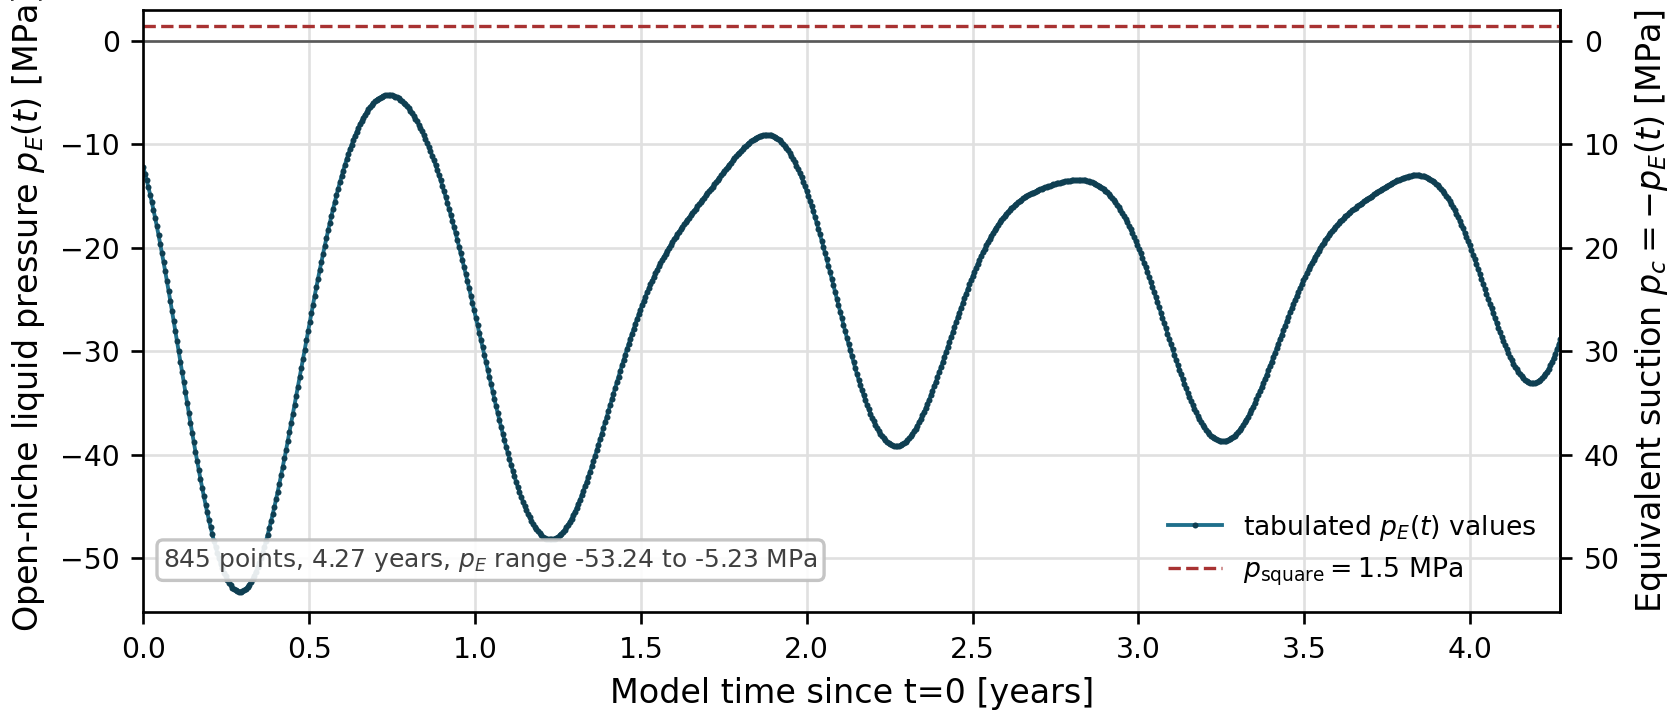
\includegraphics[width=0.9\textwidth]{resources/figures/open_niche_pressure_curve.png}
  \caption{Tabulated open-niche pressure boundary data \(p_E(t)\) prescribed on
  \(\Gamma_E\).  The markers are the 845 XML values used by the active OGS setup.
  The left axis shows liquid pressure; the right axis shows the equivalent suction
  under \(p_c=-p_E(t)\).  The dashed line marks the constant square-boundary
  pressure \(p_\square=1.5\,\mathrm{MPa}\) for scale.}
  \label{fig:open-niche-pressure-curve}
\end{figure}

The figure is an input diagnostic, not a measurement-provenance closure.  It shows
the numerical forcing passed to OGS.  The source sensors, filtering, time-origin
convention, and uncertainty of this boundary-data vector remain the boundary-input
gate recorded in Section~\ref{sec:question-inventory-gates}.

The mechanical boundary inventory is component-wise kinematic support on the outer
square,
\begin{equation}
  u_x=0 \quad \text{on } \Gamma_A\cup\Gamma_B,
  \qquad
  u_y=0 \quad \text{on } \Gamma_C\cup\Gamma_D,
  \label{eq:mechanical-bc}
\end{equation}
with natural tangential components and natural niche traction in the current model.
\revadd{12}{On the niche boundary this means no prescribed mechanical displacement
and no separately applied mechanical traction.  It does not remove hydraulic
coupling: the prescribed niche liquid pressure still enters the momentum balance
through the Bishop/Biot pore-pressure term in \eqref{eq:momentum}.}{\annCommentTwelve}
The thermal boundary is \(\TT=298.15\,\mathrm{K}\) on the thermal support used by the
OGS setup.  The initial conditions are
\begin{equation}
  \uu(\xx,0)=\bm{0},\qquad
  \pl(\xx,0)=1.5\times10^6\,\mathrm{Pa},\qquad
  \TT(\xx,0)=298.15\,\mathrm{K}.
  \label{eq:initial-state}
\end{equation}
The pressure expression in the XML contains a vertical term multiplied by zero.
Consequently, the active initial pressure field is spatially uniform and does not
encode a drained near-niche post-excavation pressure field.

\section{OGS System Realization}
\label{sec:ogs-system}

\subsection{Project Blocks and Process Variables}
\label{sec:ogs-project-blocks}

The OGS realization is the \texttt{THERMO\_RICHARDS\_MECHANICS} process in
\path{01_processes_TRM.xml}.  The project assigns polynomial order 2 to displacement
and order 1 to pressure and temperature.  The same process block exposes
\texttt{velocity}, \texttt{saturation}, \texttt{sigma}, \texttt{epsilon}, and
\texttt{swelling\_stress} as secondary variables.  Gravity is off because
\texttt{specific\_body\_force} is \texttt{0 0}
\citep[``Process variables'']{OpenGeoSysTRMDocs}
\citep[initial and boundary-condition structure]{OpenGeoSysProcessVariablesDocs}.

The time-loop files bind this process to Backward Euler time discretization, fixed
time stepping, and the nonlinear solver \texttt{basic\_newton}.  The nonlinear solver
is a Newton solver with at most 150 iterations and delegates linear systems to
\texttt{general\_linear\_solver}, which uses \texttt{PardisoLU}.  The convergence
criterion is component-wise \(\Delta x\) in the \(L^2\) norm, with absolute tolerance
\(10^{-10}\) and relative tolerance \(10^{-8}\) for each primary-variable component.
These settings define the numerical realization of the frozen TRM equations; they do
not change the governing equations or the material-field choices.

Table~\ref{tab:ogs-field-mapping} maps the mathematical quantities to the OGS
blocks, parameters, mesh fields, and output arrays.  This table is the bridge between
the mathematical model and the file-level system.  It also prevents us from treating
an observation operator, such as NMR water content or ERT resistivity, as if it were
an OGS primary variable.

\begingroup
\small
\setlength{\tabcolsep}{3pt}
\begin{longtable}{@{}L{0.15\textwidth} L{0.27\textwidth} L{0.25\textwidth} L{0.23\textwidth}@{}}
\caption{Mapping between mathematical quantities and the OGS realization.}
\label{tab:ogs-field-mapping}\\
\toprule
Mathematical quantity & OGS block, tag, or field & Input realization & Output or downstream use\\
\midrule
\endfirsthead
\toprule
Mathematical quantity & OGS block, tag, or field & Input realization & Output or downstream use\\
\midrule
\endhead
\bottomrule
\endlastfoot
\(\uu\) &
Process variable \texttt{displacement} in \path{02_process_variables_TRM.xml}. &
Two components, polynomial order 2, initial parameter \texttt{ic\_displacement};
component-wise Dirichlet supports on the outer square. &
Current OGS VTU array \texttt{displacement}.  Mechanical observations need a
reference-zero and support operator.\\
\(\pl\) &
Process variable \texttt{pressure}. &
One component, polynomial order 1, initial parameter \texttt{ic\_pressure};
Dirichlet pressure data on the reference hydraulic supports. &
Current OGS VTU array \texttt{pressure}.  Pressure measurements and RH-derived
suction require sign and reference-pressure conventions.\\
\(\TT\) &
Process variable \texttt{temperature}. &
One component, polynomial order 1, initial parameter \texttt{ic\_temperature};
Dirichlet temperature parameter \texttt{bc\_temperature\_outside}. &
Current OGS VTU array \texttt{temperature}.  In the active parametrization it is
constrained to \(T_0=298.15\,\mathrm{K}\), so thermal gradients and temperature-change
terms vanish.\\
\(\KK\) &
Medium property \texttt{permeability}, parameter \texttt{k\_i}. &
Current OGS \texttt{MeshElement} field \texttt{k\_i\_rd} on the projected bulk mesh.
The source package also contains a constant tensor fallback. &
Not a dynamic state variable.  Observation operators sample or average the mesh
field for pulse-test permeability comparisons.\\
\(\por\) &
Medium property \texttt{porosity}, parameter \texttt{phi}. &
Current OGS \texttt{MeshElement} field \texttt{n\_rd}; current field package is
spatially constant at \(0.105\). &
Current OGS VTU array \texttt{porosity}.  Used with saturation to form
\(\theta=\por\Sl\).\\
\(\Sl\) &
Medium property \texttt{saturation} and process secondary variable. &
Computed by \texttt{SaturationVanGenuchten} from \(\pc=-\pl\); not prescribed as a
primary variable. &
Current OGS VTU array \texttt{saturation}.  Main state field for water-content
observation operators.\\
\(k_{\mathrm{rel}}\) &
Medium property \texttt{relative\_permeability}. &
Computed by the OGS van Genuchten relative-permeability law; fixed parameters in
the reference setup. &
Usually not exported as a required VTU field.  It affects pressure and saturation
through Darcy mobility.\\
\(\vl\) and \(\ql\) &
Secondary variable \texttt{velocity}. &
Computed from \(\KK\), \(k_{\mathrm{rel}}\), \(\mu_l\), and \(\grad\pl\). &
Available from the process if requested.  Flux residuals require an explicit
Darcy-velocity versus pore-velocity convention.\\
\(\sig\), \(\eps\), swelling stress &
Secondary variables \texttt{sigma}, \texttt{epsilon}, and \texttt{swelling\_stress}. &
Computed from the orthotropic elasticity law, Bishop/Biot coupling, thermal strain,
and saturation-dependent swelling. &
Available from the process if requested.  Current HM measurements remain gated by
prestress, excavation, and reference-zero decisions.\\
\(p_E(t)\) &
\texttt{open\_niche\_seasonal} and \texttt{open\_niche\_seasonal\_curve}. &
\texttt{CurveScaled} parameter with unit scaling factor 1.0. &
Active boundary forcing in the reference setup.  Its measurement provenance,
filtering, and uncertainty remain open.\\
\end{longtable}
\endgroup


\subsection{Mesh and Boundary Supports}
\label{sec:mesh-boundary-supports}

The transferred project uses boundary submeshes \path{cd-a_left},
\path{cd-a_right}, \path{cd-a_top}, \path{cd-a_bottom}, and \path{cd-a_niche4}.
Figure~\ref{fig:domain-bc} gives the schematic notation for these supports.  The
figure is only a notation aid; the boundary-condition table below gives the
model-facing mapping to XML tags and prescribed data.

\begin{center}
  \centering
  \begin{tikzpicture}[scale=0.72, every node/.style={font=\small}]
  \coordinate (A) at (-5,-5);
  \coordinate (B) at (5,-5);
  \coordinate (C) at (5,5);
  \coordinate (D) at (-5,5);

  \fill[gray!6] (A) rectangle (C);
  \draw[thick] (A) rectangle (C);

  \draw[red!70!black, very thick] (-5,-5) -- (-5,5);
  \draw[red!70!black, very thick] (5,-5) -- (5,5);
  \draw[red!70!black, very thick] (-5,5) -- (5,5);
  \draw[red!70!black, very thick] (-5,-5) -- (5,-5);

  \node[red!70!black, anchor=east] at (-5.25,0) {$\Gamma_A$};
  \node[red!70!black, anchor=west] at (5.25,0) {$\Gamma_B$};
  \node[red!70!black, anchor=south] at (0,5.25) {$\Gamma_C$};
  \node[red!70!black, anchor=north] at (0,-5.25) {$\Gamma_D$};

  \draw[orange!80!black, line width=1.1pt] (0,0) circle (1.25);
  \node[orange!80!black, align=center] at (0,0)
    {$\Gamma_E$};

  \foreach \y in {-3.6,-2.2,-0.8,0.8,2.2,3.6} {
    \draw[-{Stealth[length=2.0mm]}, blue!70!black] (-5.35,\y) -- (-5.02,\y);
    \draw[-{Stealth[length=2.0mm]}, blue!70!black] (5.35,\y) -- (5.02,\y);
  }
  \foreach \x in {-3.6,-2.2,-0.8,0.8,2.2,3.6} {
    \draw[-{Stealth[length=2.0mm]}, blue!70!black] (\x,5.35) -- (\x,5.02);
    \draw[-{Stealth[length=2.0mm]}, blue!70!black] (\x,-5.35) -- (\x,-5.02);
  }

  \draw[dashed, gray!70] (-5,0) -- (5,0);
  \draw[dashed, gray!70] (0,-5) -- (0,5);
\end{tikzpicture}

  \captionof{figure}{Schematic boundary-condition map for the reference
  two-dimensional model.  The outer square boundary is denoted by
  \(\Gamma_A\cup\Gamma_B\cup\Gamma_C\cup\Gamma_D\), and the niche boundary is
  denoted by \(\Gamma_E\).}
  \label{fig:domain-bc}
\end{center}

\begin{center}
\begingroup
\scriptsize
\renewcommand{\arraystretch}{1.12}
\setlength{\tabcolsep}{3pt}
\captionof{table}{Boundary-set notation, XML tags, and prescribed mechanical/hydraulic data.}
\label{tab:boundary-conditions}
\begin{tabular}{@{}L{0.15\textwidth} L{0.26\textwidth} L{0.22\textwidth} L{0.29\textwidth}@{}}
\toprule
Boundary set & XML tag name and parameter & Mechanical BC & Hydraulic BC\\
\midrule
\(\Gamma_A\) &
\path{cd-a_left}; \path{bc_displacement}; reference square-pressure parameter
\path{bc_pressure_outside}. &
Dirichlet \(u_x=0\); tangential component natural. &
Dirichlet \(\pl=p_\square\), \(p_\square=1.5\times10^6\,\mathrm{Pa}\).\\
\(\Gamma_B\) &
\path{cd-a_right}; \path{bc_displacement}; reference square-pressure parameter
\path{bc_pressure_outside}. &
Dirichlet \(u_x=0\); tangential component natural. &
Dirichlet \(\pl=p_\square\), \(p_\square=1.5\times10^6\,\mathrm{Pa}\).\\
\(\Gamma_C\) &
\path{cd-a_top}; \path{bc_displacement}; \path{bc_top_pressure}. &
Dirichlet \(u_y=0\); tangential component natural; \path{load_top} inactive. &
Dirichlet \(\pl=p_\square\), \(p_\square=1.5\times10^6\,\mathrm{Pa}\).\\
\(\Gamma_D\) &
\path{cd-a_bottom}; \path{bc_displacement}; reference square-pressure parameter
\path{bc_pressure_outside}. &
Dirichlet \(u_y=0\); tangential component natural. &
Dirichlet \(\pl=p_\square\), \(p_\square=1.5\times10^6\,\mathrm{Pa}\).\\
\(\Gamma_A\cup\Gamma_B\) &
\path{cd-a_left}, \path{cd-a_right}. &
Compact mechanics notation: \(u_x=0\). &
Part of the square hydraulic Dirichlet boundary
\(\pl=p_\square\).\\
\(\Gamma_C\cup\Gamma_D\) &
\path{cd-a_top}, \path{cd-a_bottom}. &
Compact mechanics notation: \(u_y=0\). &
Part of the square hydraulic Dirichlet boundary
\(\pl=p_\square\).\\
\(\Gamma_\square=\Gamma_A\cup\Gamma_B\cup\Gamma_C\cup\Gamma_D\) &
\path{cd-a_left}, \path{cd-a_right}, \path{cd-a_top}, \path{cd-a_bottom}. &
Outer-box kinematic support, component-wise. &
Dirichlet \(\pl=p_\square=1.5\times10^6\,\mathrm{Pa}\) on all four sides of the
outer square in the reference boundary inventory.  Checked OGS XML attachment
for left/right/bottom remains a consistency gate.\\
\(\Gamma_E\) &
\path{cd-a_niche4}; \path{open_niche_seasonal};
\path{open_niche_seasonal_curve}; \path{pressure_scaling_factor}. &
No prescribed displacement or traction in the active boundary-condition block. &
Dirichlet \(\pl=p_E(t)\).  The curve has 845 tabulated values, spans \(0\) to
\(1.3482\times10^8\) s, and ranges from about \(-5.23\) to \(-53.24\) MPa.\\
\bottomrule
\end{tabular}
\endgroup
\end{center}


The table states the required reference boundary inventory: constant hydraulic
Dirichlet data on all four sides of the square and a time-dependent niche pressure
curve.  In the checked \path{02_process_variables_TRM.xml}, the named pressure
conditions are the constant \path{bc_top_pressure} entry and the
\path{open_niche_seasonal} entry on \path{cd-a_niche4}.  Thus the live modelling
distinction is simple: the open niche uses the seasonal curve, while the square
boundary is treated as fixed-pressure support.  The remaining open question is not
which boundary is seasonal, but whether the seasonal curve's source timestamps and
model-time origin match the measurement time axes used later.

\subsection{Material Fields and OGS Inputs}
\label{sec:material-fields-ogs-inputs}

The OGS parameter block can define constants, functions, curve-scaled data, and mesh
element or mesh node fields
\citep[sections ``CurveScaled'', ``Function'', and ``MeshElement and MeshNode'']{OpenGeoSysParametersDocs}.
The current OGS workflow uses \texttt{MeshElement} parameters for intrinsic
permeability and porosity.  The intrinsic permeability tensor is supplied through
\texttt{k\_i\_rd}; this is the local workflow field whose magnitude is varied in
the present inversion examples.  Candidate changes enter OGS through this current-run
mesh field or through explicit XML/input replacement, not through hidden edits to
the governing equations.  Porosity is supplied through \texttt{n\_rd}, but in
the current field package all cells have value \(0.105\).  This is a mesh-field
representation of fixed support, not a porosity inversion.
\revnote{32}{\pdfAnnComment{15}{spise pro nas}{Hydraulic conductivity is kept as a
derived quantity from intrinsic permeability, relative permeability, density,
viscosity, and head convention; it is not an independent field in the first
workflow.}}
\revnote{33}{\pdfAnnComment{16}{spise pro nas}{The saturation and retention answer
defines \(\Sl\), \(S_e\), residual saturation, and their roles in storage,
relative permeability, swelling, and water-content post-processing.}}
\revadd{34}{A heterogeneous porosity field would be a new modelling decision, not a
property already varied by the current \texttt{n\_rd} package.}{\pdfAnnComment{17}{ma
smysl heterogenni \(n\)?}{The reviewed text now answers this as a modelling policy:
the current porosity support is fixed, and heterogeneous \(n\) needs independent
evidence or an explicit modelling decision.}}
\revnote{35}{\pdfAnnComment{18}{spsie pro nas?}{The storativity row states that
storage follows from porosity, saturation derivative, liquid compressibility,
density, and volumetric coupling; no separate storativity field is varied.}}
\revadd{36}{Likewise, \(\alpha_B=1\) and the Bishop exponent one are checked XML
choices; the paper does not claim that this is the only valid HM setup.}{\pdfAnnComment{19}{je
\(\alpha_b = 1\) dobra volba pro nas setup?}{The answer is a model-change
decision: the current model uses the checked XML values, while changing them needs
mechanical evidence and a scenario decision.}}
\revadd{13}{The current local workflow varies only the permeability tensor field
across candidate inverse runs; other families remain present in OGS but are not
fitted in this pass.}{\annCommentThirteen}
\revadd{7}{If the permeability tensor components encode bedding anisotropy through a
rotation, the bedding angle and coordinate convention must be stated explicitly.
The present text therefore treats bedding orientation as a structural prior and a
tensor-parameterization gate, not as a hidden fact implied by component values.}{\annCommentSeven}

\begingroup
\small
\setlength{\tabcolsep}{3pt}
\begin{longtable}{@{}L{0.17\textwidth} L{0.27\textwidth} L{0.24\textwidth} L{0.22\textwidth}@{}}
\caption{Material and constitutive fields in the active model or tied to OGS fields.}
\label{tab:material-fields}\\
\toprule
Field & Material meaning & Relation to other fields & OGS role in the current workflow\\
\midrule
\endfirsthead
\toprule
Field & Material meaning & Relation to other fields & OGS role in the current workflow\\
\midrule
\endhead
\bottomrule
\endlastfoot
Intrinsic permeability tensor \(\KK(\xx)\) &
Clay/EDZ effective Darcy mobility before relative permeability and viscosity are
applied.  It is the main hydraulic material field for the present inversion. &
Hydraulic conductivity is derived from \(\KK\), liquid density, viscosity, relative
permeability, and saturation state; it is not an independent base field here. &
Current OGS \texttt{MeshElement} field \texttt{k\_i\_rd}.  Current release gates allow
permeability magnitude changes while tensor shape remains staged.\\
Porosity \(\por(\xx)\) &
Effective pore-volume fraction used by the OGS continuum model. &
Water content is \(\theta=\por\Sl\) only for the mobile/OGS liquid storage; NMR,
ERT, and Taupe/TDR may also see bound/interlayer water or calibration offsets. &
Current OGS \texttt{MeshElement} field \texttt{n\_rd}, fixed at \(0.105\) in the
current field package.  Not released as an unknown yet.\\
Saturation \(\Sl\) and retention \(S_l(p_c)\) &
Liquid occupancy of the OGS pore space, governed by a retention law. &
\(p_c=-\pl\) under the active gas/reference convention; the same law controls
storage derivative and water-content output. &
Fixed OGS van Genuchten saturation law with \(S_{lr}=0.1\), \(S_{gr}=0\),
exponent \(m=0.45\), and \(p_b=10\,\mathrm{MPa}\).\\
Relative permeability \(k_{\mathrm{rel}}(\Sl)\) &
Reduction of liquid mobility in unsaturated conditions. &
Multiplies \(\KK/\mu_l\) in Darcy velocity; should not be fitted independently of
retention without a release decision. &
Fixed OGS van Genuchten relative-permeability law with the same residual
saturations, exponent \(0.45\), and minimum \(10^{-25}\).\\
Biot and Bishop coupling &
Poromechanical coupling between pore pressure, saturation, and stress. &
\(\alpha_B=1\) and \(b(\Sl)=\Sl\) reduce the pore-stress scaling to \(\Sl\pl\II\). &
Fixed XML parameter \texttt{biot}=1 and \texttt{BishopsPowerLaw} exponent 1.\\
Orthotropic elasticity \(\CC\) &
Directional stiffness of Opalinus Clay in the 2D mechanical approximation. &
Controls stress/displacement response together with pore pressure, saturation,
swelling, and any prestress assumption. &
Fixed orthotropic linear elasticity: \(E=(13.8,6.0,13.8)\) GPa,
\(G=(4.79,2.46,4.79)\) GPa, \(\nu=(0.44,0.22,0.44)\).  Mechanical release is gated.\\
Swelling stress contribution &
Saturation-driven mechanical source representing swelling response. &
Coupled to saturation and constrained by mechanical boundary assumptions; can mimic
deformation from pressure changes if released prematurely. &
Active fixed saturation-dependent swelling law with \(1.0\) MPa swelling
pressures in all directions and limits \(S_l\in[0.1,1]\).\\
Thermal and liquid properties &
Solid/liquid storage, conductivity, density, viscosity, and isothermal coupling
context. &
In the full XML, liquid density depends linearly on \(T\) and \(\pl\), and thermal
expansion can enter THM coupling.  In the active reduction, \(T=T_0\), so only the
pressure part of density varies. &
Fixed XML constants/laws.  The \texttt{CTE}=1254.74 value is a provenance caveat and
should not be interpreted as a calibrated thermal-expansion coefficient.\\
Fault, fracture, crack, and EDZ fields &
Structural features that may localize permeability, porosity, stiffness, or aperture. &
Measured aperture could imply hydraulic aperture or localized permeability only after
scale, clay-contact, and 3D-to-2D projection assumptions are accepted. &
Not an active OGS geometry/material class in this chapter.  They remain structural
priors, masks, scenarios, or qualitative diagnostics until source data are resolved.\\
Time-dependent material fields &
Possible healing, sealing, fracture closure, or EDZ evolution over the multi-year
experiment. &
Could appear as \(K(\xx,t)\), \(n(\xx,t)\), retention changes, or boundary/input
changes, but may be confounded with forcing and saturation state. &
Excluded from the first static permeability-field workflow.  Release requires
same-support repeated evidence and state-output diagnostics.\\
\end{longtable}
\endgroup


The material-field question is therefore not only which constants appear in XML.
For each field we need to know its material meaning, whether it is a base field or a
derived field, whether it is independent enough to vary, and how OGS consumes it.
In the first workflow, \(\KK(\xx)\) is the only varied base material field.
Hydraulic conductivity, water content, storativity, resistivity, and flux are
derived from \(\KK\), \(\por\), \(\Sl\), fluid properties, and observation
operators \citep[Darcy law and effective-storage equation]{OpenGeoSysTRMDocs}
\citep[Sec.~3, Eq.~3]{WaterContentEDZ2024}.
No separate storativity field is varied in this setup.  Storage behaviour is
already represented through porosity, the saturation derivative, liquid
compressibility/density, and hydro-mechanical volumetric coupling in
\eqref{eq:mass-balance} and \eqref{eq:isothermal-mass-balance}.
\revnote{41}{\pdfAnnComment{24}{pozdejsi faze nebo od zacatku?}{Fault, crack, and
EDZ geometry are kept from the start as structural context and possible priors or
scenario fields, but they are not active discrete OGS geometry or varied material
classes in the first permeability-field workflow.}}

\subsection{Initial Conditions, Time Grid, and Outputs}
\label{sec:initial-time-output}

The initial-condition XML entries realize \eqref{eq:initial-state}.  The time-step
file comments identify \(t=0\) with 18 September 2019.  The active grid starts at
zero seconds, uses fixed Backward Euler stepping, and ends at
\(1.4\times10^8\,\mathrm{s}\).  The first block uses 365 steps of 864,000 s, and
the second block uses 365 steps of 1,314,900 s.  The output schedule is intended to
match the monthly ERT cadence after the first output, as stated in comments in
\path{05_time_loop_TRM.xml} and \path{05_1_fixed_timestepping.xml}.

\begingroup
\small
\setlength{\tabcolsep}{3pt}
\begin{longtable}{@{}L{0.13\textwidth} L{0.19\textwidth} L{0.20\textwidth} L{0.38\textwidth}@{}}
\caption{Initial conditions used by the active TRM process.}
\label{tab:initial-conditions}\\
\toprule
Variable & XML parameter & Active value & Interpretation and modelling gate\\
\midrule
\endfirsthead
\toprule
Variable & XML parameter & Active value & Interpretation and modelling gate\\
\midrule
\endhead
\bottomrule
\endlastfoot
\(\uu(\xx,0)\) & \texttt{ic\_displacement} & \((0,0)\,\mathrm{m}\) &
The model starts from zero displacement on the already open two-dimensional geometry.
No excavation/driving phase is represented explicitly.\\
\(\pl(\xx,0)\) & \texttt{ic\_pressure} &
\(1.5\times 10^{6}\,\mathrm{Pa}\) everywhere &
The XML function contains a vertical term multiplied by zero, therefore the active
initial liquid pressure is spatially uniform.  This remains a gate for pressure
history: no post-excavation drained niche field is encoded.\\
\(\TT(\xx,0)\) & \texttt{ic\_temperature} &
\(298.15\,\mathrm{K}\) &
The model is initialized at \(T_0\).  Together with the \texttt{bulk\_all}
temperature Dirichlet condition, this enforces homogeneous constant temperature in
the active parametrization.\\
\(\sig_0\) & \texttt{ic\_sigma0} &
Defined but inactive &
The file defines in-situ stress-like expressions, but the process XML comments out
the initial-stress reference.  Prestress is therefore a provenance question, not an
active initial condition in the present run.\\
\end{longtable}
\endgroup


This initial state is a numerical post-excavation state.  It is not a simulation of
the initial excavation or gradual niche unloading.  In mechanics, \texttt{ic\_sigma0}
is defined but not connected as active initial stress, and \texttt{load\_top} remains
inside a commented top-load block.  In hydraulics, the initial pressure is uniform
and does not reconstruct near-niche drainage from nearby holes, RH/suction, or
direct pressure measurements.  Early transients may therefore mix physical drainage
with adjustment from the prescribed initial state.
\revadd{21}{The uniform initial pressure is therefore a checked numerical input, not
a claim that the nearby experiments prove spatially uniform post-excavation
drainage.}{\pdfAnnComment{4}{je to dobre? viz Simciny experimenty}{The answer is
gated: the XML value is clear, but the paper does not promote it to a
measurement-validated drainage state.}}
\revadd{22}{The elapsed time between excavation and this \(t=0\) date is not closed
by the checked OGS files; it remains part of the excavation-reference gate.}{\pdfAnnComment{5}{kolik
casu je od exkavace?}{The paper now states that the model start date is known from
the time-step comments, while the excavation-reference interval is not closed by the
available OGS files.}}
\revnote{23}{\pdfAnnComment{6}{chceme si vyjasnit}{The initial-pressure answer
explicitly says that post-excavation near-niche drainage is not encoded unless an
external drainage field or measurement-based initialization is supplied.}}
\revnote{24}{\pdfAnnComment{7}{chceme vyjasnit}{The question table now separates
findable measured in-situ stress values from the active XML state: published values
exist, but no active initial-stress tensor is applied.}}
\revnote{25}{\pdfAnnComment{8}{chceme vyjasnit}{The prestress-angle answer remains
a gate.  The checked sources do not close an accepted principal-stress orientation
or rotation angle for the current 2D prestress tensor.}}
\revnote{26}{\pdfAnnComment{9}{chceme vyjasnit}{The early-transient answer warns
that pressure or displacement changes can mix physical drainage with numerical
adjustment from the prescribed post-excavation initial state.}}

\begin{figure}[htbp]
  \centering
  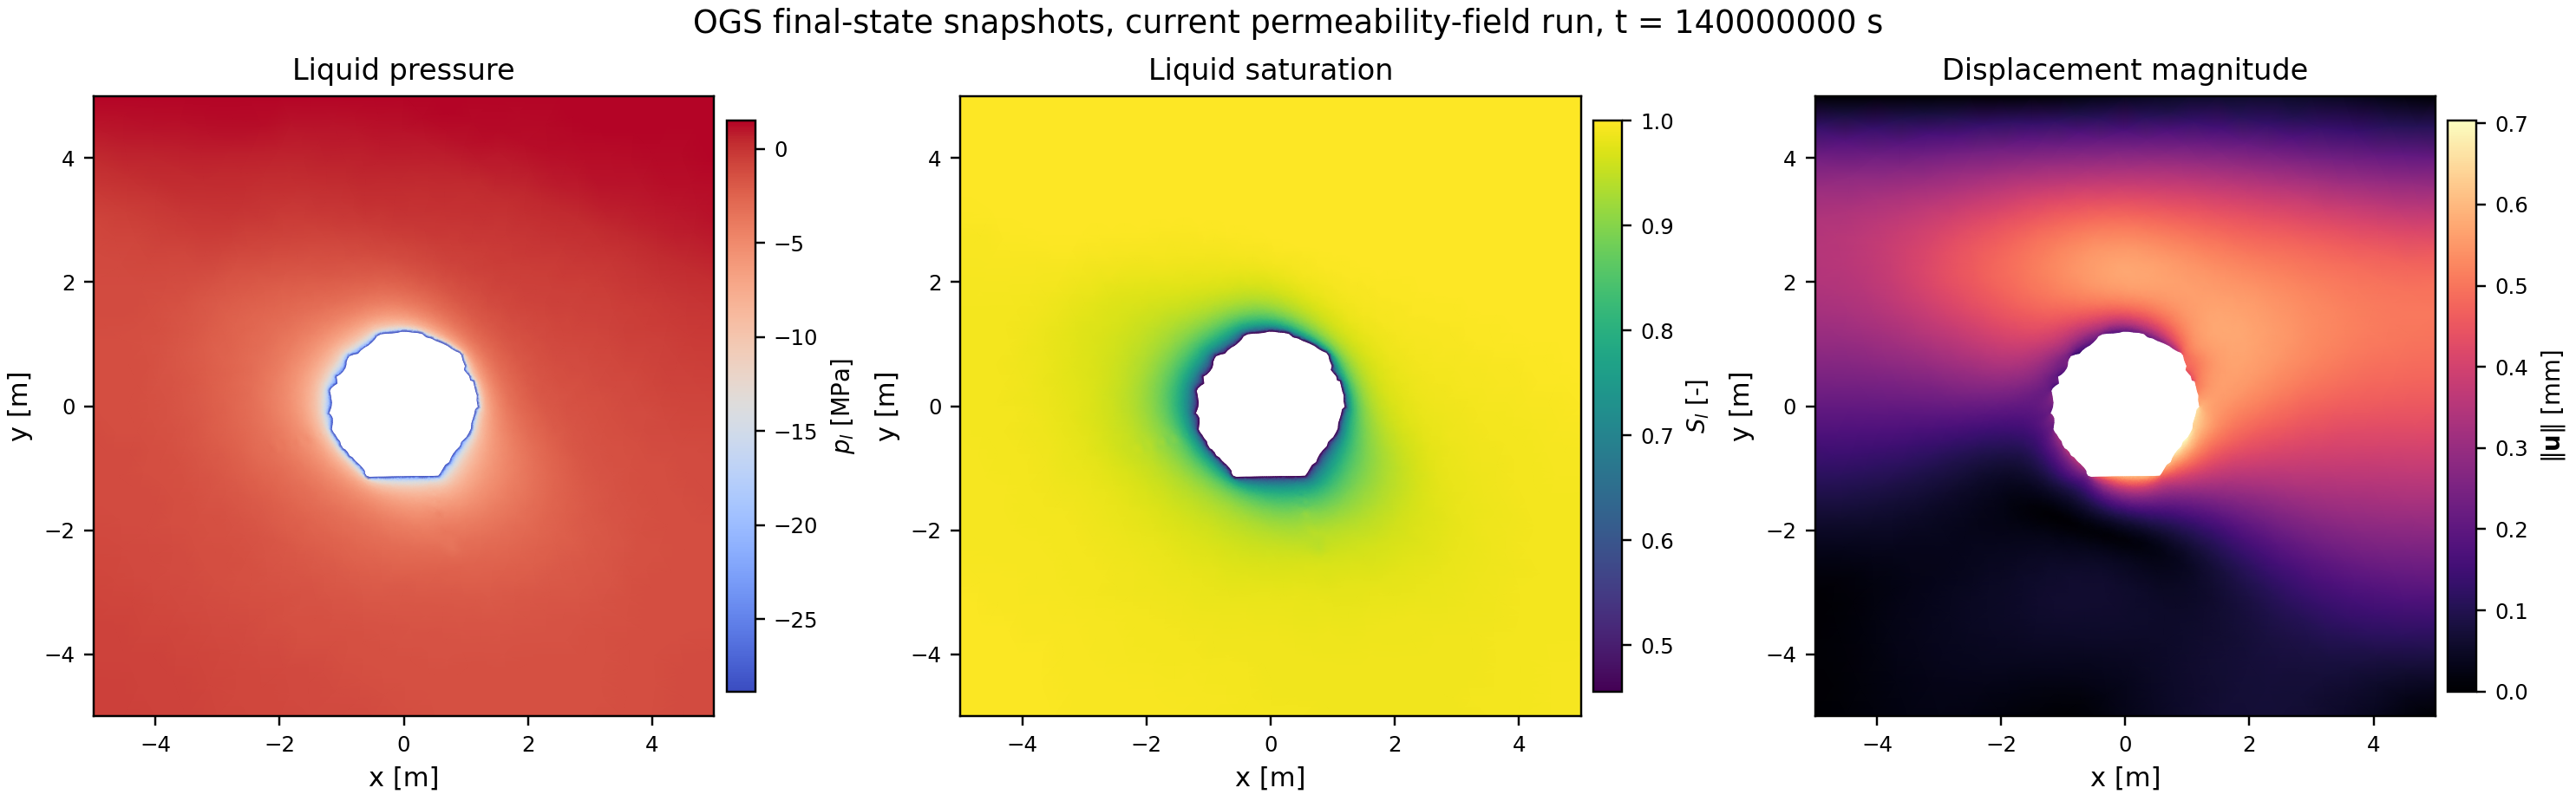
\includegraphics[width=\textwidth]{resources/figures/ogs_solver_snapshots.png}
  \caption{Final-state snapshots from the current permeability-field OGS run at
  \(t=1.4\times10^8\) s.  The panels show liquid pressure, liquid saturation, and
  displacement magnitude from the current OGS VTU output.  The figure is a diagnostic
  visualization of the active solver state; it is not itself a measurement residual.}
  \label{fig:ogs-solver-snapshots}
\end{figure}

\subsection{Model Outputs and Observation Operators}
\label{sec:model-outputs-observation-operators}

The OGS output layer must stay separate from measurement-specific observation
operators.  The current OGS workflow requests pressure, saturation, temperature,
displacement, and porosity.  These arrays are model states or fixed support fields,
not residuals by themselves.  \revadd{15}{A residual is the signed model-data
mismatch, for example \(r=H(u)-d\), after the observation operator \(H\) has fixed
the measured quantity, support, time mapping, unit convention, reference state, and
uncertainty.}{\annCommentFifteen} For a Gaussian likelihood this becomes a
posterior-informing term only after the uncertainty is stated, e.g.
\((H_i(u)-d_i)/\sigma_i\) or \(-\tfrac12(H_i(u)-d_i)^2/\sigma_i^2\) for datum
\(i\).  Permeability comparisons are a separate case: they sample or average the
input tensor field, because permeability is not a dynamic state output.

\begingroup
\small
\setlength{\tabcolsep}{3pt}
\begin{longtable}{@{}L{0.17\textwidth} L{0.21\textwidth} L{0.25\textwidth} L{0.27\textwidth}@{}}
\caption{Model outputs and observation-facing quantities.}
\label{tab:outputs-observation-ties}\\
\toprule
Quantity & OGS status & Measurement tie & Required operator or gate\\
\midrule
\endfirsthead
\toprule
Quantity & OGS status & Measurement tie & Required operator or gate\\
\midrule
\endhead
\bottomrule
\endlastfoot
\(\pl\) &
Primary variable and current OGS VTU output. &
Direct pressure or mini-piezometer data, pressure-boundary checks, and pressure
diagnostics. &
Reference convention, elevation/head conversion, gauge/absolute convention, and 2D
projection error must be explicit.\\
\(\uu\) &
Primary variable and current OGS VTU output. &
Geoscope, crackometer, levelling, extensometer, laser-scan, and deformation screens. &
Reference-zero, sign convention, support geometry, and whether displacement can be
used as a hard residual are unresolved.\\
\(\TT\) &
Primary variable and current OGS VTU output. &
Constrained field for the present isothermal workflow. &
Thermal residuals are not active; \(\TT=T_0\) fixes thermal gradients and
temperature-change terms.\\
\(\Sl\) &
Secondary variable and current OGS VTU output. &
Water-content streams after transformation: NMR, Taupe/TDR, and ERT-derived moisture. &
Must be converted to \(\theta=\por\Sl\) or another accepted observable; bound-water and
calibration policies remain gates.\\
\(\por\) &
Material field and current OGS VTU output. &
Support for \(\theta=\por\Sl\), not an observed active unknown yet. &
Current \(\por=0.105\) support must be retained unless NMR/ERT/Taupe policies justify a
porosity release.\\
\(\KK\) or \(e^\top\KK e\) &
Input field, not a state output unless sampled from mesh data. &
Pulse-test permeability/transmissibility interpretations. &
Interval orientation, support averaging, gas/slip correction, and duplicate-support
likelihood policy are required.\\
\(\vl\), \(\ql\) &
Secondary velocity available from OGS; flux can be derived. &
Hydraulic diagnostics and possible flow-rate checks if such data are supplied. &
Use Darcy velocity, not pore velocity, unless an observation operator explicitly
requires division by \(\por\Sl\).\\
\(\sig,\eps\), swelling stress &
Secondary variables available from the process. &
Mechanical plausibility, crack/deformation interpretation, and the prestress gate. &
Initial stress and excavation unloading are not active; mechanical conclusions need
separate staged-model or post-excavation assumptions.\\
\(\theta=\por\Sl\) &
Post-processing product. &
NMR and Taupe/TDR water-content comparison; ERT if transformed through a
water-content/resistivity relation. &
Decide absolute versus bias-corrected versus trend/anomaly comparison and handle
bound/interlayer water.\\
Resistivity or log-resistivity proxy &
Observation-model product, not an OGS state variable. &
ERT inversion fields. &
Requires Archie/clay-specific transform, pore-water conductivity/salinity treatment,
surface conduction, anisotropy, support aggregation, and covariance policy.\\
\end{longtable}
\endgroup


\section{Model-facing Question Inventory and Proposed Answers}
\label{sec:question-inventory-gates}

This section keeps only the questions that still define an unresolved model choice
or require external confirmation.  Resolved facts are no longer repeated as
questions here; they are stated in the preceding prose and in
Tables~\ref{tab:boundary-conditions}, \ref{tab:ogs-field-mapping}, and
\ref{tab:outputs-observation-ties}.
\revreplaceonly{11}{Which pressure Dirichlet conditions are attached in the checked
OGS XML?}{Checked XML pressure-boundary attachment gate}{\annCommentEleven}
\revreplaceonly{14}{Is permeability an OGS state output?}{How should permeability be
compared when it is an input field?}{\annCommentFourteen}
\revnote{27}{\pdfAnnComment{10}{asi jasne}{The active process and primary variables
are already stated in the OGS-input question table: TRM with displacement, pressure,
and temperature variables.}}
\revnote{28}{\pdfAnnComment{11}{asi jasne?}{The source hierarchy answer states that
the checked OGS XML defines the active run and that documentation or notation
mismatches are treated as gates.}}
\revnote{29}{\pdfAnnComment{12}{jasne, mozna se zeptat na tolerance?}{The numerical
answer includes Backward Euler, fixed time stepping, Newton iteration limit,
component-wise convergence tolerances, and PardisoLU.  Any stricter tolerance
justification would be a solver-study request.}}
\revnote{30}{\pdfAnnComment{13}{ok, pokud nechceme menit model}{The inactive-term
answer records the current fixed baseline: no active vapor phase, source term,
initial stress, or top load unless the model is intentionally changed.}}

\begingroup
\footnotesize
\renewcommand{\arraystretch}{1.16}
\setlength{\tabcolsep}{4pt}
\definecolor{qaQuestionBg}{gray}{0.93}
\definecolor{qaPolicy}{HTML}{6F42C1}
\definecolor{qaGate}{HTML}{D97706}
\definecolor{qaCaveat}{HTML}{B42318}
\newcommand{\qaStatus}[2]{\textcolor{#1}{\textbf{#2}}}
\newcommand{\qaPair}[4]{%
  \rowcolor{qaQuestionBg}%
  \multicolumn{2}{@{}L{0.96\textwidth}@{}}{\textbf{Question.} #3}\\*%
  \textbf{Answer.} & #4\\%
  \addlinespace[0.42em]%
}
\newcommand{\qaSubtable}[1]{%
  \par\Needspace{8\baselineskip}\medskip\noindent\textbf{#1}\par\smallskip%
}

\captionof{table}{Live model-facing questions after resolved setup facts have been
moved into the model text and mapping tables.  Questions are shaded light grey and
answers are unshaded.}
\label{tab:explicit-question-answers}

\qaSubtable{Hydraulic Boundary-Data Provenance}
\begin{longtable}{@{}L{0.18\textwidth} L{0.76\textwidth}@{}}
\toprule
\qaPair{qaGate}{Gate}{\qid{Q006} Which timestamp and time-origin convention produced the active niche curve \(p_E(t)\)?}{The active OGS input is clear: the open niche uses
\path{open_niche_seasonal}, while the square boundary is treated as fixed-pressure
support.  The open query is the source time axis.  The provider should confirm the
source timestamps, time zone or date convention, interpolation/smoothing, mapping
to OGS \(t=0\), and whether the ERT-suggested time shift seen in initial tests also
applies to the boundary curve.}
\bottomrule
\end{longtable}

\qaSubtable{Initial State, Excavation, and Prestress}
\begin{longtable}{@{}L{0.18\textwidth} L{0.76\textwidth}@{}}
\toprule
\qaPair{qaGate}{Gate}{\qid{Q012} Does the initial pressure encode post-excavation drainage near the niche?}{No.  The current input has no heterogeneous initial drainage field from
RH/suction, direct pressure, nearby boreholes, or excavation history.  A
measurement-based initialization needs an accepted source field and date before it
can replace the uniform value.}
\qaPair{qaCaveat}{Caveat}{\qid{Q013} Does the model simulate staged excavation or gradual unloading?}{No.  The computation starts from the already-open 2D geometry, with
\(\uu(\xx,0)=\bm{0}\), no active initial stress tensor, and no active top load.
The elapsed time from excavation to the model start date is not closed by the
checked OGS files.}
\qaPair{qaGate}{Gate}{\qid{Q014} Which prestress magnitude, angle, and excavation reference should be used if prestress is activated?}{Published CD-A modelling sources give stress-magnitude evidence, but no accepted
active prestress tensor for this run.  The water-content modelling paper reports
\(\sigma_h=3\,\mathrm{MPa}\) and \(\sigma_v=7\,\mathrm{MPa}\)
\citep[Sec.~3]{WaterContentEDZ2024}; the GETE modelling paper lists
\(\sig_0=-(5,5,7)\times10^6\,\mathrm{Pa}\)
\citep[modelling Table~2]{Ziefle2022GETE}.  The current XML does not apply either
value, and a usable 2D prestress still needs principal directions or rotation angle,
component order, sign convention, value choice, and an excavation-reference state.}
\bottomrule
\end{longtable}

\qaSubtable{OGS Inputs and Material-Field Questions}
\begin{longtable}{@{}L{0.18\textwidth} L{0.76\textwidth}@{}}
\toprule
\qaPair{qaGate}{Gate}{\qid{Q025} Are mechanical parameters fitted now?}{No.  Orthotropic elasticity, \(\alpha_B=1\), Bishop exponent 1, and
saturation-dependent swelling are active but fixed.  Elastic-parameter fitting
requires a later internal modelling decision, hydro-mechanical residuals, and a
settled prestress/excavation reference state.}
\qaPair{qaGate}{Gate}{\qid{Q027} Is there expert consensus that material fields should evolve in time during the multi-year experiment?}{The current OGS baseline uses time-independent permeability, porosity, retention,
and mechanical material fields.  Expert input is needed on whether clay sealing,
fracture closure/opening, EDZ healing, or other time-dependent material evolution is
physically expected strongly enough to justify adding fitted time-dependent fields
rather than explaining the trends by boundary forcing, saturation state, or spatial
heterogeneity.}
\bottomrule
\end{longtable}

\qaSubtable{Model Time and Output Operators}
\begin{longtable}{@{}L{0.18\textwidth} L{0.76\textwidth}@{}}
\toprule
\qaPair{qaGate}{Gate}{\qid{Q032} How are output times tied to observations or boundary curves?}{The run starts at \(t=0\), identified by comments as 18 September 2019, and ends
at \(1.4\times10^8\,\mathrm{s}\).  Measurements require an explicit
date-to-model-time conversion, tolerance, and interpolation or matching rule.  This
gate is now especially important because initial ERT tests suggest a possible
time-axis shift.}
\bottomrule
\end{longtable}

\qaSubtable{Material and Structural Questions}
\begin{longtable}{@{}L{0.18\textwidth} L{0.76\textwidth}@{}}
\toprule
\qaPair{qaGate}{Gate}{\qid{Q042} Does the same bedding angle control mechanics, permeability, and electrical anisotropy?}{The cited structural evidence supports bedding orientation as important context for
permeability candidates, but it does not prove that Darcy, mechanical, electrical,
and prestress orientations must share one hard angle.  Tensor rotations should
state their bedding-angle, prestress-angle, and coordinate conventions explicitly
rather than hiding the choices inside component values.}
\qaPair{qaGate}{Gate}{\qid{Q044} How should faults, cracks, and EDZ features be classified here?}{They are not active discrete OGS geometry or separate material classes in this
chapter.  They can become structural priors, masks, equivalent fields, or
scenarios only after their source geometry, scale, aperture meaning, and
3D-to-2D projection are defined.}
\bottomrule
\end{longtable}
\endgroup

